\section{Related Work}
\label{sec:related}
\begin{figure*}[t]
    \centering
      \resizebox{1.0\textwidth}{!}
      {
    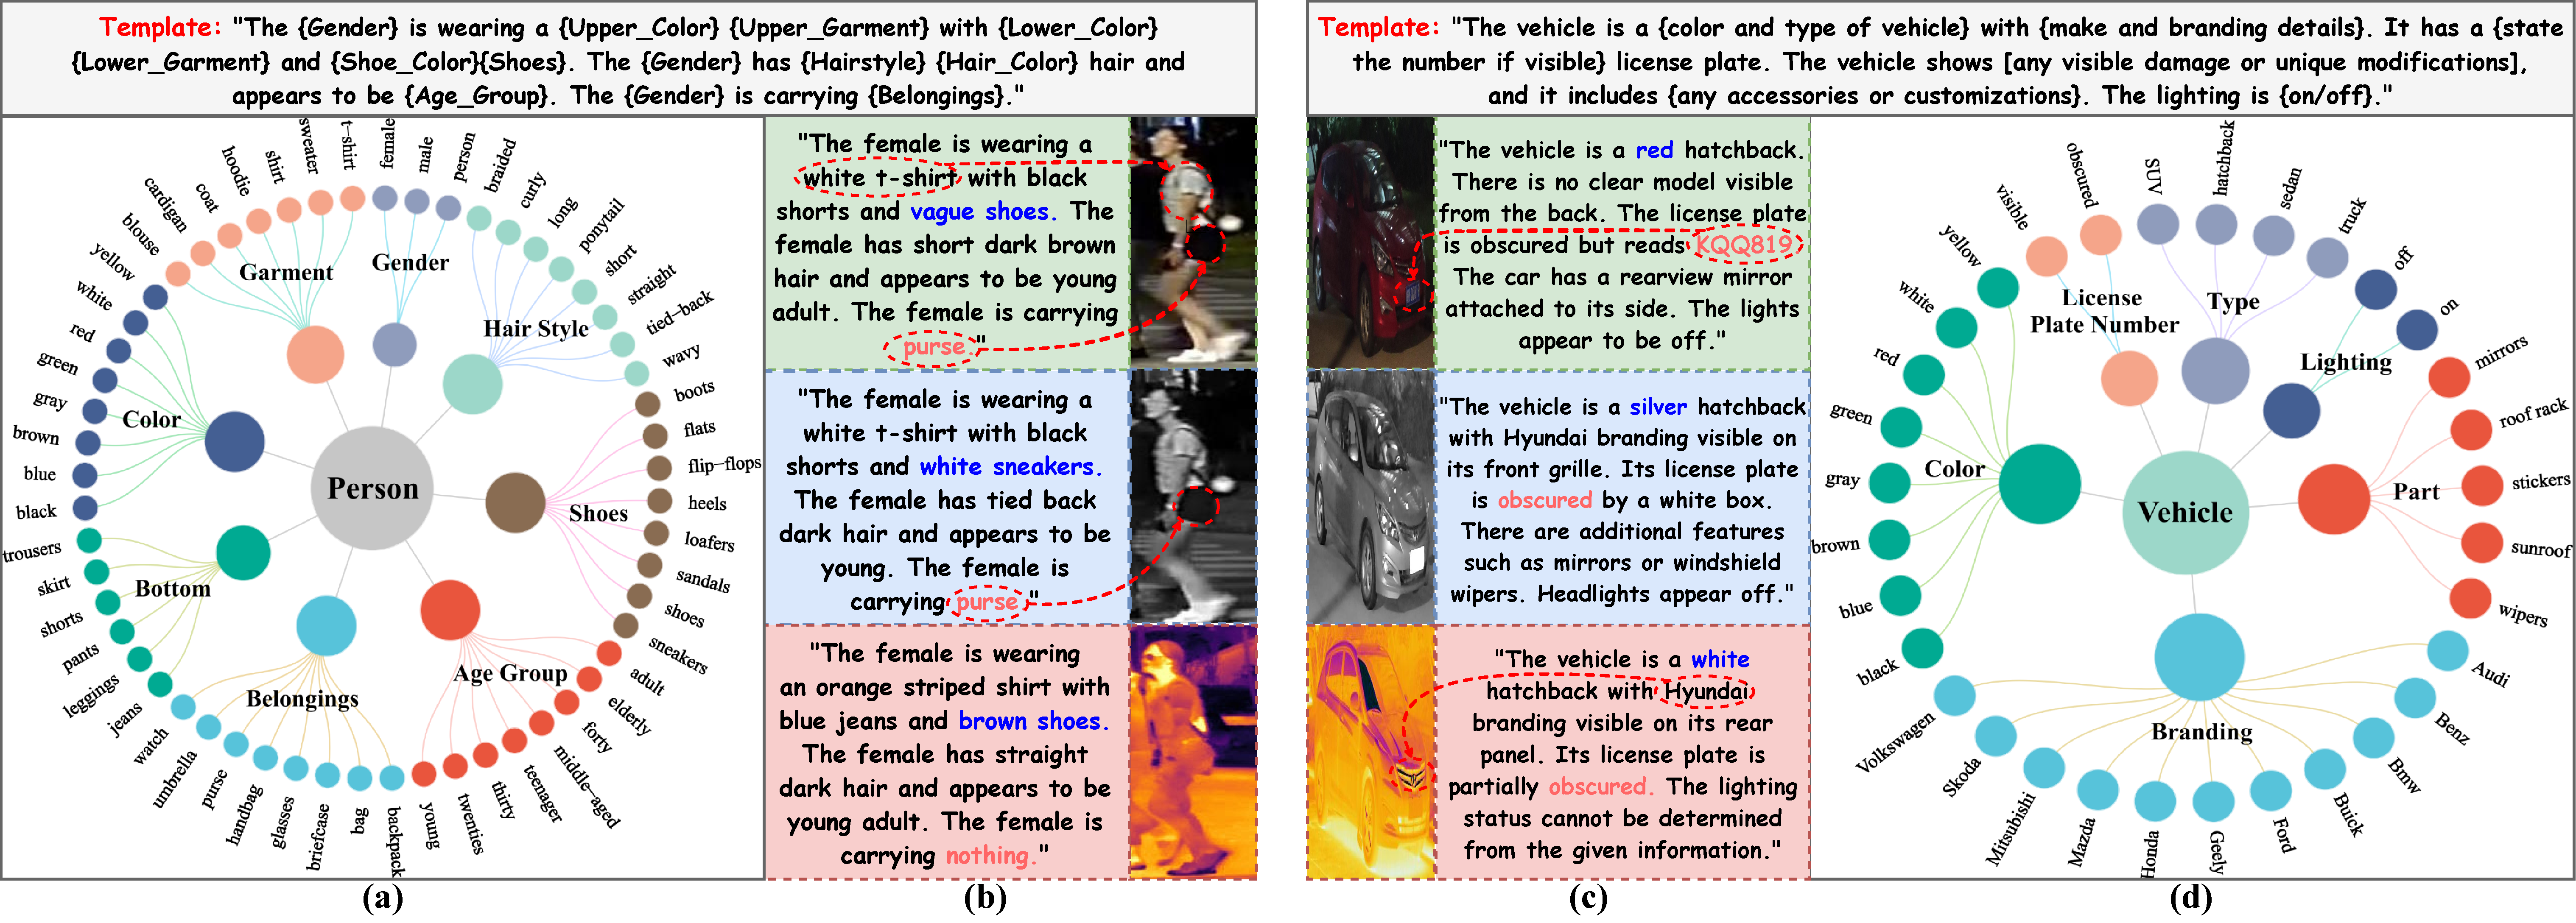
\includegraphics[width=30\linewidth]{sec/img/Dataset_Example.pdf}
    }
    \vspace{-6mm}
     \caption{The upper row presents the template used to annotate our dataset.
     %
     The lower row provides detailed information about the annotated dataset.
     %
     (a) Category statistics for our annotated person ReID dataset.
     %
     (b) Example images and captions from the RGBNT201 dataset.
     %
     (c) Category statistics for our annotated vehicle ReID dataset.
     %
     (d) Example images and captions from the MSVR310 dataset.}
    \label{fig:Dataset}
    \vspace{-2mm}
  \end{figure*}
%~~~~~~~~~~~~~~~~~~~~~~~~~~~~~~~~
\subsection{Vision-language Learning in Re-Identification}
Vision-language learning plays a pivotal role in multi-modal applications.
%
As the field advances~\cite{yu2024boosting,diao2024unveiling,yu2024llms}, there is a growing focus on exploring the interaction between visual and textual information in ReID tasks.
%
Existing methods can be broadly divided into cross-modal and multi-modal ReID. 
%
In cross-modal ReID, Text-to-Image ReID~\cite{ding2021semantically} focuses on matching text queries with image galleries. 
%
Current methods primarily emphasize feature alignment~\cite{jiang2023cross} and pre-training~\cite{tan2024harnessing}. 
%
To expand application scenarios, Zhai et al.~\cite{zhai2022trireid} combine text and sketch modalities in the query, while Chen et al.~\cite{chen2023towards} propose an uncertain Query-to-RGB retrieval model to handle missing modalities. 
%
More recently, Li et al.~\cite{li2024all} introduce flexible modality combinations and unify various uncertainties in retrieval.
%
However, these methods focus on cross-modal alignment.
%
In contrast, multi-modal ReID aims to leverage complementary information from multiple modalities, with both the query and gallery containing multi-modal data. 
%
The rise of vision-language models, particularly CLIP~\cite{radford2021learning}, has significantly advanced this area by facilitating image-text interactions. 
%
Li et al.~\cite{li2023clipreid} pioneer CLIP-ReID to learn from text templates for ReID tasks. 
%
However, the templates are not real descriptions of images, potentially restricting performance. 
%
To address this, Han et al.~\cite{han2024clip} leverage MLLMs to generate descriptions for RGB images.
%
Despite improvements, existing methods fail to tackle the challenges of generating text for multi-spectral modalities and ensuring structural consistency in the generated descriptions. 
% 
To address the above issues, we propose a structured multi-modal caption generation pipeline, enhancing the consistency of texts and providing informative annotations for multi-modal object ReID.
%
\subsection{Multi-modal Object Re-Identification}
Multi-modal object ReID gains great attention due to its robustness in real-world applications. 
%
Research primarily focuses on leveraging complementary information from different modalities. 
%
Early works emphasize effective fusion strategies~\cite{gong2021eliminate,zheng2021robust}. 
%
To enhance modality-specific learning, Wang et al.~\cite{wang2022interact} propose an interact-embed-enlarge framework to facilitate knowledge expansion. 
%
To address missing modal data, Zheng et al.~\cite{zheng2023dynamic} introduce pixel reconstruction to handle data inconsistency. 
%
Li et al.~\cite{li2020multi} use a coherence loss to guide feature fusion. 
%
Some methods further improve feature robustness with modality generation, graph learning and instance sampling~\cite{he2023graph, guo2022generative, zheng2023cross}. 
%
% The advent of vision Transformers (ViTs)~\cite{dosovitskiy2020image} shifts research toward Transformer-based architectures due to their superior generalization capabilities. 
%
%Pan et al.~\cite{pan2023progressively} and Crawford et al.~\cite{crawford2023unicat} utilize attention mechanisms to model complex cross-modal relationships.
%
Notably, Wang et al.~\cite{wang2024heterogeneous} introduce a test-time training framework to mine inter-modal interactions. 
%
Wang et al.~\cite{wang2024top} develop TOP-ReID, which employs token permutation to guide modality fusion.
%
Recently, Zhang et al.~\cite{zhang2024magic} propose diverse token selections to mitigate background noises.
%
Despite promising results, they often overlook the semantic guidance of informative text annotations.
%
Thus, we propose the IDEA framework, which incorporates generated text annotations to leverage semantic guidance.
%
This framework adaptively aggregates discriminative local information, enhancing feature robustness in complex scenarios.